\documentclass{beamer}
\usepackage{listings}
\usepackage{graphicx}
\usepackage{multirow}
\lstset{
%language=C,
frame=single, 
breaklines=true,
columns=fullflexible
}
\usepackage{subcaption}
\usepackage{url}
\usepackage{tikz}
\usepackage{tkz-euclide} % loads  TikZ and tkz-base
%\usetkzobj{all}
\usetikzlibrary{calc,math}
\usepackage{float}
\newcommand\norm[1]{\left\lVert#1\right\rVert}
\renewcommand{\vec}[1]{\mathbf{#1}}
\usepackage[export]{adjustbox}
\usepackage[utf8]{inputenc}
\usepackage{amsmath}
\usetheme{Boadilla}

\title{Research Paper Presentation}
\author{Vanga Aravind Shounik}
\date{CS20BTECH11055}
\begin{document}
%
\begin{frame}
    \titlepage
\end{frame}

\begin{frame}
    \begin{block}{Title}
    Probabilistic Approach for Intrusion Detection System - FOMC Technique
    \end{block}
    \begin{block}{Authors}
    \begin{enumerate}
        \item A.S.Aneetha - Anna University, Chennai
        \item S.Bose - Anna University, Chennai
    \end{enumerate}
    \end{block}
\end{frame}

\begin{frame}{What is Intrusion Detection System?}
\begin{enumerate}
    \item An Intrusion Detection System (IDS) is a device or software application that monitors a network for malicious activity or policy violations.
    \item IDS can be either Hardware and/or Software which is capable of detecting any malicious or unusual activities in the network 
    \item There are 2 types of IDS 
    \begin{enumerate}
        \item Host based IDS
        \item Network based IDS
    \end{enumerate}
\end{enumerate}

\end{frame}
\begin{frame}
\begin{block}{Host Based IDS}
        Host Based IDS consists of an agent on a host which identifies intrusions by analyzing file system modifications, system calls etc.
\end{block}
\begin{block}{Network Based IDS}
    In a Network IDS environment, 2 types of detection system namely 
    \begin{enumerate}
        \item Signature Based Detection:\\
            It compares ongoing observations with patterns of well known attacks.\\
            It cannot detect a new type of attack.
        
        \item Anomaly Based Detection:\\
            It builds a model based on the normal profile and any deviation from this is signaled an anomaly.
    \end{enumerate}
\end{block}
\end{frame}

\begin{frame}{Anomaly Based Detection}

    Here, new attacks can also be detected but the time taken to analyse it is high.\\
    It has 2 stages:
\begin{enumerate}
    \item It builds the model using training normal traffic profile.
    \item It is evaluated using testing traffic profile.
\end{enumerate}
Most anomaly based IDS detects the attacks after they cause serious damage to the system.\\
It is necessary to to design an Intrusion Detection Model which is capable of predicting the anomalous events in network before it causes serious damage to the system. 
\end{frame}
\begin{frame}{First Order Markov Chain}
\begin{block}{Definition}
A Markov chain is a first order discrete time stochastic process that predicts the future by analyzing traditional characteristic from one state to another state. This model analyses the operation of the system with finite number of states and it's state transition property.
\end{block}
\begin{block}{Properties}
The property of First Order Markov Chain says that the state of a system at time $n+1$ depends only on the state at time $n$ but not on $n-1$,$n-2$..
\begin{align}
    P(S_{n+1}=i_{n+1}|S_n=i_n,...S_0=i_0)=P(S_{n+1}=i_{n+1}|S_n=i_n)
\end{align}
\begin{enumerate}
    \item $n$ and $n+1$ represents the sampling time at which the states are defined and the time interval between $n$ and $n+1$ can be either regular or irregular.
\end{enumerate}
\end{block}
\end{frame}

\begin{frame}{First Order Markov Chain continued...}
Here, we take
\begin{align}
    P(S_{n+1}=i_{n+1}|S_n=i_n)=P(S_{n+1}=j|S_n=i)=p_{ij}
\end{align}
Where $p_{ij}$ is the probability of state transition from state $i$ to state $j$ in the time interval of $n$ and $n+1$\\
The Markov model can be defined for the system with $k$ number of finite states using the probability transition matrix 
\begin{align}
    P=\begin{bmatrix}
p_{11}&p_{12}&...&p_{1k}\\
p_{21}&p_{22}&...&p_{2k}\\
.&.&...&.\\
.&.&...&.\\
p_{k1}&p_{k2}&...&p_{kk}
\end{bmatrix}   \label{eq3}
\end{align}
with the constraint,
\begin{align}
    \sum_{j=1}^k p_{ij}=1   \label{eq4}
\end{align}
\end{frame}

\begin{frame}{First Order Markov Chain continued...}
There is another matrix $Q$ which is initial probability distribution matrix.
\begin{align}
    Q=\begin{bmatrix}
q_1&q_2&...&q_k
\end{bmatrix}^T \label{eq5}
\end{align}
These matrices are calculated from the past observed data events made on the system. The data observations $X_o, X_i, ...., X_{N-1}$ are taken from the system at time $n =0,1, ...., N-1$.
\begin{align}
    p_{ij}&=N_{ij}/N_i\\
    q_i&=N_i/N \text{, for }i,j=1,...k 
\end{align}
$N_{ij}$ is the number of observation pairs $X_n$ and $X_{n+1}$with $X_n$ in the state $i$ and $X_{n+1}$is in state $j$,\\
$N_i$ is the number of data items in the state $i$ and\\
$N$ is the total number of data item used to build the system.\\
The joint probability for a given sequence of $T$ states $X_{n-T+1}...,X_n$ at time $n-T+1,..n$ is
\begin{align}
    P(S_{t-N},S_{t-N+1}...S_t)=q_{S_{t-N}}\Pi_{i=N}^1 P_{S_{t-i}S_{t-i+1}}
\end{align}
\end{frame}

\begin{frame}{Proposed Framework}
The proposed FOMC model for anomaly intrusion detection in the network based on first order Markov chain process is discussed.\\
Since the framework is designed to detect anomalous activities in the network, it has two phases
\begin{enumerate}
    \item Training Phase
    \item Testing Phase
\end{enumerate}
There are 3 steps in Training Phase,
\begin{enumerate}
    \item Pre-Processing
    \item Defining the states
    \item Building FOMC Model
\end{enumerate}
\end{frame}

\begin{frame}{Proposed Framework continued...}
\begin{block}{Proposed Framework}
In pre-processing step, data cleaning and transformation are carried out to the form needed for model development, finite number of states are defined with processed data using clustering approach and FOMC model is build with state transition matrix and initial probability distribution.\\
\end{block}
\begin{block}{Proposed Framewok continued...}
In the testing phase the test data undergoes the same pre-processing as in training phase, the deviation factor is calculated to classify test data belongs to normal or abnormal state. The probability of event occurrence for the specified time period T for the test data is calculated based on FOMC model. If the probability of event occurrence value is lesser than the predefined threshold, then the test data is considered as anomaly event otherwise it is considered as the normal event.
\end{block}

\end{frame}

\begin{frame}{Pre-Processing Step}
\begin{enumerate}
    \item The data contains many unnecessary profiles which are needed to be removed so that the results will not be biased towards the repeated set of profiles.
    \item The data need to be transformed into the form suitable for developing the model, by removing the labels and assigning numerical equivalent for categorical and symbolic attributes to perform the mathematical operations. 
    \item Normalization has to be carried out for the features using Min Max technique so that all values can be represented in a given range which in this case is [0,1]
\end{enumerate}
\begin{align}
    V_{i(new)}=\frac{V_{i(old)}-V_{min}}{V_{max}-V_{min}}
\end{align}
Where $V_{i(new)}$ - new normalized value for $i^{th}$ record of that attribute,\\
$V_{max}$ - maximum value of that attribute and\\
$V_{min}$ - minimum value of that attribute.
\end{frame}

\begin{frame}{Defining the States}
\begin{enumerate}
    \item After pre-processing the data, we will define states using k-means clustering.
    \item Each cluster formed by k-means clustering is defined as a state in FOMC model.A new state called outlier state is defined to represent any anomaly in the test data.
    \item Since only normal profiles are used in the Markov model building, the outlier state is needed for representing unusualness in the test data along with the normal states formed by clustering.
\end{enumerate}
\end{frame}

\begin{frame}{Building FOMC Model}
FOMC model is build based on the state transition probability matrix, P, computed using \eqref{eq3} using the constraint in \eqref{eq4} along with initial probability distribution using \eqref{eq5}.\\
Here, In the FOMC model apart from defined states, new outlier state is also added. The new probability transition matrix is computed by considering the outlier state along the normal states defined by clustering process. \\
The outlier state row and column of the matrix are computed based on the assumptions made.
\begin{enumerate}
    \item The probability of state transition from a normal to outlier is considered as minimum, assumed as zero.
    \item The probability of state transition from outlier to outlier state is also less, assumed as zero.
    \item The probability of the state transition from the outlier to normal state is proportional to the number of data points belong to each state. It is same as initial probability distribution Q.
\end{enumerate}

\end{frame}

\begin{frame}{Deviation Factor Analysis}
Since normal records are only used in the Markov model, the outlier state is needed to represent unusualness in the test data in addition to the normal states.
So outlier state is introduced in the probability transition matrix to define the abnormality in the test traffic profile.\\
We introduce a new variable called Deviation Factor(DF) which is computed as
\begin{align}
    DF(x)=\frac{\sqrt{\sum_{i=1}^k d(C_i-x)^2}}{K}
\end{align}
Where $d(C_i-x)$ is Euclidean distance which is calculated as
\begin{align}
    d(C_i-x)=\sqrt{\sum_{k=1}^n(C_{ik}-x_k)^2}
\end{align}
Where $n$ is the number of attributes.
\end{frame}
\begin{frame}{Deviation Factor Analysis continued}
    We write another variable $d_m$ which is given by
\begin{align}
    d_m=min_{0\leq i\leq k}\{d(C_i-x)\}
\end{align}
The Decision rule for the deviation factor is that if the $d_m$ value of the data point is greater than the $DF(x)$, then the data point belongs to outlying state, otherwise, it belongs the normal state which is closest, i.e, if $d_m >DF(x)$, it lies in the outlier state.
\end{frame}

\begin{frame}{Anomaly Detection System}
\begin{enumerate}
    \item The objective of the FOMC model is to test the observed traffic profile for any anomaly, based on probability of event occurrence of that observation.
    \item As the intrusions are made in steps the changes in the behavioral pattern are identified from sequences of transition of the data from state to state, which may also help in suspecting the traffic. 
    \item The probability of event occurrences for the specific sequence of states is calculated and it is compared with the sequence of states has one or more abnormal activities. 
    \item In the testing phase, the probability of event occurrences is calculated using the equation given in (8) for the specified T size.
    \item The probability of event occurrence value of the test data is considered as normal if the value is greater than the threshold otherwise anomaly to the degree of that probability.
\end{enumerate}
\end{frame}

\begin{frame}{Results and Discussions}
\begin{block}{Dataset Description}
\begin{enumerate}
    \item We use the network traffic profile of KDD Cup'99 benchmark Dataset.
    \item It consists of 41 attributes.
    \item In building phase only the normal profiles are utilized, whereas testing has done in two ways, one is with the normal profile alone but not used in model development and other one is test data with fifty percent of attack profile along with fifty percent of normal profile.
    \item Both training and testing data are pre-processed by assigning numeric values for the categorical attributes and attribute normalization process which equalizes all the attributes irrespective for their greater or lesser original attribute values.
\end{enumerate}
\end{block}
\end{frame}
\begin{frame}{Results and Discussions continued...}
\begin{enumerate}
    \item The first step of FOMC model design is defining the network states using the k-means clustering technique based on which the actual detection system is developed. 
    \item The proposed system uses N-fold cross validation method for evaluating the performance of the model and the best results are considered as outputs.
    \item Here N is set to 10 for the entire training traffic profile.
\end{enumerate}
\end{frame}
\begin{frame}{Graphs of the Observations}
\begin{figure}[h!]
    \centering
    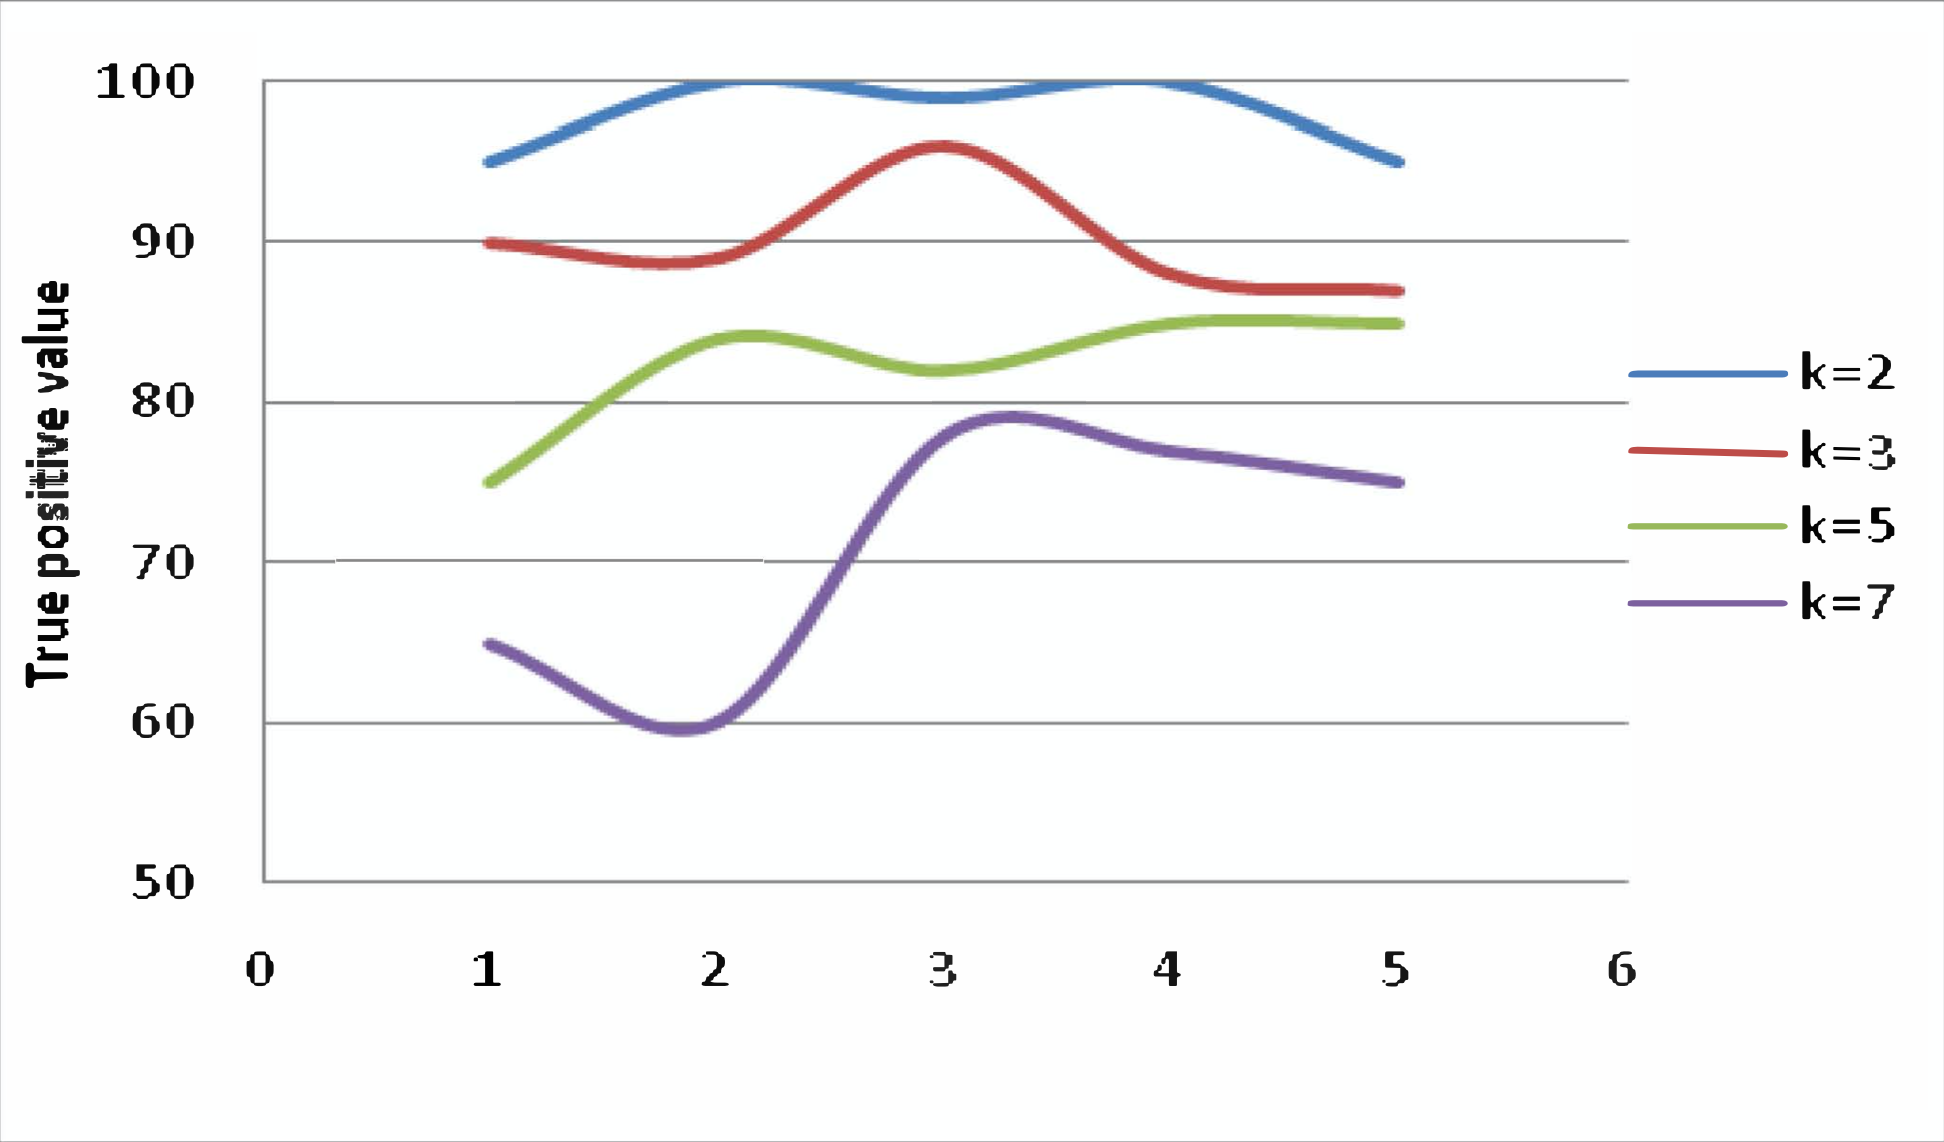
\includegraphics[scale=0.2]{fig1.png}
    \caption{True positive rate Vs States}
    \label{fig1}
\end{figure}
From this, we can see that when the states are 2, the system gives consistent performance. Whereas in the case of seven, five and three the system performance varies much.
\end{frame}

\begin{frame}{Results and Conclusions continued...}
\begin{table}[h!]
    \centering
    \hline
    \hline
    \begin{tabular}{|c|c|c|c|c|c|c|}
        \multirow{2}{2em}{S.No} & \multicolumn{2}{|c|}{K=2} & \multicolumn{2}{|c|}{K=3} & \multicolumn{2}{|c|}{K=7}\\
        & Testset1 & TestSet2 & Testset1 & TestSet2 & Testset1 & TestSet2\\
        \hline
        1. & 95\% & 100\% & 90\% & 100\% & 65\% & 80\% \\
        2. & 100\% & 90\% & 89\% & 82\% & 60\% & ---\\
        3. & 97\% & 96\% & 78\% & 75\% & 85\% & 78\% \\
        4. & 99\% & 100\% & 96\% & 88\% & 82\% & 80\% \\
        5. & 94\% & 100\% & 78\% & 96\% & 60\% & 78\% \\
        6. & 90\% & 80\% & 60\% & 72\% & 72\% & 80\% \\
        7. & 100\% & 96\% & 88\% & 74\% & 80\% & 84\% \\
        8. & 97\% & 100\% & 79\% & 82\% & 63\% & 66\% \\
        9. & 90\% & 100\% & 67\% & 83\% & 55\% & ---\\
        10. & 95\% & 100\% & 79\% & 90\% & 75\% & 75\% \\
        \hline
        \hline
    \end{tabular}
    \caption{Detection Rates for Number of States}
    \label{tab:my_label}
\end{table}
Here, we can see that testdata 2 performance is better than testdata 1 even though there are 50\% Dos attacks included.
\end{frame}
\begin{frame}
\begin{block}{Conclusion}
\begin{enumerate}
    \item The probabilistic approach of analyzing intrusion in the network traffic has been proposed.
    \item The probabilistic approach deploys first order Markov chain process to predict the anomalous activities in the network.
    \item The traffic is suspected as abnormal if the computed probability of event occurrences, based on state transition matrix and initial probability distribution, of the test data is lesser than the predefined threshold value, otherwise it is considered as normal traffic.
\end{enumerate}
\end{block}
\end{frame}
\begin{frame}
\begin{center}
    \Huge{Thank You}
\end{center}
\end{frame}
\end{document}